\documentclass[12pt]{article}

\usepackage{sbc-template}
\usepackage{graphicx,url}
\usepackage[utf8]{inputenc}
\usepackage[brazil]{babel}
\usepackage[latin1]{inputenc}  

     
\sloppy

\title{Arquitetura Híbrida para Armazenamento de Dados em Internet das Coisas}
\author{Luiz G. Fritsch\inst{1}}


\address{Universidade Federal dos Pampas
  (Unipampa)\\
 Alegrete -- RS -- Brazil
  \email{fritsch.guilherm3@gmail.com}
}

\begin{document} 

\maketitle

\begin{abstract}
  This meta-paper describes the style to be used in articles and short papers
  for SBC conferences. For papers in English, you should add just an abstract
  while for the papers in Portuguese, we also ask for an abstract in
  Portuguese (``resumo''). In both cases, abstracts should not have more than
  10 lines and must be in the first page of the paper.
\end{abstract}
     
\begin{resumo} 
  
\end{resumo}


\section{Introdução}

Internet das coisas tem como princípio a conectividade de dispositivos, não apenas como em geral acontece hoje com computadores e smartphones, mas com todo tipo de dispositivo, sejam eles sensores como um sensor de umidade do solo,  ou até mesmo objetos do nosso cotidiano, como torradeiras, cafeteiras e geladeiras.\\
Estes dispositivos que antes eram simples objetos estáticos e com uma função específica, agora se tornam cada vez mais “inteligentes” e acabam sendo usados como uma fonte de dados que podem ser analisados para melhorar o nosso dia-a-dia.\\
Esta alta variedade de dispositivos geram dados dos mais diversos tipos e em um volume muito grande. Surge então o problema de descobrir um local adequado não só para se armazenar estes dados, mas para também que seja eficiente quando for necessário realizar consultas. (Elaborar mais)\\
Para este problema de armazenamento, surgem soluções como o armazenamento em nuvem, que, segundo a empresa Amazon, “é um modelo de computação em nuvem que armazena dados na Internet por meio de um provedor de computação na nuvem, que gerencia e opera o armazenamento físico de dados como serviço”[1]. Temos também o armazenamento In The Edge, que se resume em armazenar os dados nos próprios dispositivos para reduzir os custos de banda larga com transmissão de dados. \\
Como engatar DB`s NoSQL aqui?\\
“Bases de dados NoSQL (originalmente se referindo a "no SQL": "não SQL" ou "não relacional", posteriormente estendido para Not Only SQL - Não Somente SQL) é um termo genérico que representa os bancos de dados não relacionais“[2]. Estas bases de dados surgiram a partir da necessidade de grandes empresas como Google, Facebook e Amazon (Não se limitando a apenas estas) tratarem de grandes volumes de dados.
Outra solução também são os modelos híbridos de armazenamento que utilizam de várias soluções como estas para resolver um problema.\\
(Descrever mais todas estas soluções, talvez?)
Neste trabalho, será apresentado uma proposta de arquitetura híbrida de armazenamento para internet das coisas, utilizando múltiplas bases de dados NoSQL

\section{Motivação} \label{sec:Motivação}


\section{Objetivos gerais}



\section{Objetivos específicos}



\section{Fundamentação teórica}



\section{Metodologia}



\section{Resultados Preliminares}



\section{Figures and Captions}\label{sec:figs}




\begin{figure}[ht]
\centering
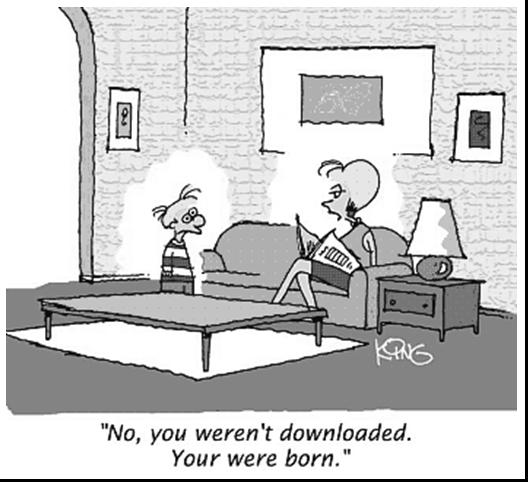
\includegraphics[width=.5\textwidth]{fig1.jpg}
\caption{A typical figure}
\label{fig:exampleFig1}
\end{figure}

\begin{figure}[ht]
\centering
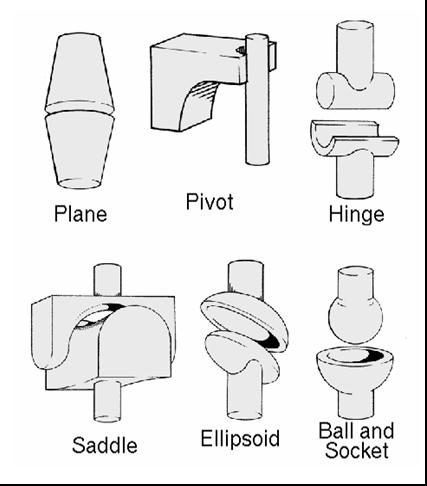
\includegraphics[width=.3\textwidth]{fig2.jpg}
\caption{This figure is an example of a figure caption taking more than one
  line and justified considering margins mentioned in Section~\ref{sec:figs}.}
\label{fig:exampleFig2}
\end{figure}



\begin{table}[ht]
\centering
\caption{Variables to be considered on the evaluation of interaction
  techniques}
\label{tab:exTable1}
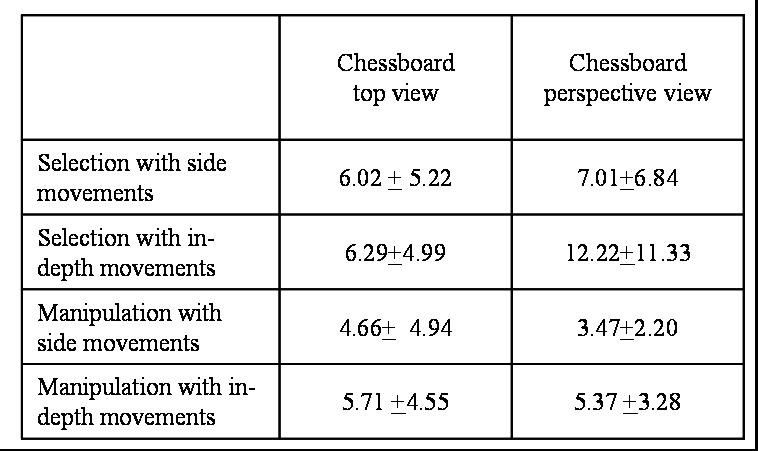
\includegraphics[width=.7\textwidth]{table.jpg}
\end{table}

\section{Images}



\section{References}

Bibliographic references must be unambiguous and uniform.  We recommend giving
the author names references in brackets, e.g. \cite{knuth:84},
\cite{boulic:91}, and \cite{smith:99}.

The references must be listed using 12 point font size, with 6 points of space
before each reference. The first line of each reference should not be
indented, while the subsequent should be indented by 0.5 cm.

\bibliographystyle{sbc}
\bibliography{sbc-template}

\end{document}
